\section*{拟阵}\addcontentsline{toc}{section}{拟阵}
许多组合优化问题可表述如下：给定一个集合系统 $(E,\F)$，即有限集 $E$ 及某 $\F\subseteq2^E$，再给定费用函数 $c:\F\to\R$，求 $\F$ 中费用最小或最大的元素。
以下默认 $c(X)=\sum_{e\in X}c(e)$。

以下只考虑 $\F$ 描述独立系统（即对子集封闭）乃至拟阵的组合优化问题。

第1节引入独立系统和拟阵，并说明许多组合优化问题可在这一框架中描述。拟阵有若干等价的公理系统（第2节），以及一种有趣的对偶关系（第3节）。拟阵之所以重要，主要在于可以用简单的贪心算法在拟阵上进行优化。第4节分析贪心算法，随后转向两个拟阵之交上的优化问题。第5节说明此问题及其带权形式可在多项式时间内求解。这也解决了以独立集覆盖一个拟阵的问题，见第6节。

\sect{1\quad 独立系统与拟阵}
\st{定义1} 若集合系统 $(E,\F)$ 满足下列条件，就称其为\textbf{独立系统}（independence system）：
\begin{description}
\item[(M1)] $\varnothing\in\F$；
\item[(M2)] 若 $X\subseteq Y\in\F$，则 $X\in\F$。
\end{description}
$\F$ 的元素称为\textbf{独立集}，$2^E\setminus\F$ 的元素称为\textbf{相关集}。极小相关集称为\textbf{回路}（circuit），极大独立集称为\textbf{基}（basis）。对 $X\subseteq E$，$X$ 的极大独立子集称为 $X$ 的基。

\st{定义2} 设 $(E,\F)$ 是独立系统。对 $X\subseteq E$，定义 $X$ 的\textbf{秩}为
\[r(X):=\max\{|Y|:Y\subseteq X,\ Y\in\F\}.\]
并定义 $X$ 的\textbf{闭包}为 $\sigma(X):=\{y\in E:r(X\cup\{y\})=r(X)\}$。

以下以 $(E,\F)$ 表示独立系统，以 $c:E\to\R$ 表示费用函数。我们着重考虑以下两个问题。
\alg{独立系统上的最大化问题}
\textbf{实例：}独立系统 $(E,\F)$ 和函数 $c:E\to\R$。\par
\textbf{任务：}求 $X\in\F$，使 $c(X):=\sum_{e\in X}c(e)$ 最大。
\par\smallskip\noindent\textbf{说明。}不妨设 $c$ 取值非负，因为从 $X\in\F$ 中删除负权元素仍得到独立集，且费用增加，因此可先将底集限制在非负权元素上。此时，任意独立集 $X$ 都可扩充为一个基 $B\supseteq X$，且 $c(B)\ge c(X)$，故只须在基中寻找最大值。
\alg{独立系统上的最小化问题}
\textbf{实例：}独立系统 $(E,\F)$ 和函数 $c:E\to\R$。\par
\textbf{任务：}求一个基 $B$，使 $c(B)$ 最小。

这里对实例的说明还不十分精确。集合 $E$ 和费用函数 $c$ 像通常一样显式给出。但 $\F$ 通常并不通过列出其全部元素来给出，而是假定有一个预言机：给定 $F\subseteq E$，它能判定 $F\in\F$ 是否成立。第4节将再次讨论这个问题。

下面的例子表明，许多组合优化问题确实具有上述两种形式之一。
\begin{enumerate}[label=(\arabic*)]
\item \textbf{最大权独立集问题。}给定图 $G$ 及权函数 $c:V(G)\to\R$，求 $G$ 中权重最大的独立集 $X$。这里 $E=V(G)$，$\F=\{F\subseteq E:F\text{ 在 }G\text{ 中独立}\}$。
\item \textbf{旅行商问题（TSP）。}给定完全无向图 $G$ 及权函数 $c:E(G)\to\R_+$，求 $G$ 中权重最小的哈密顿回路。这里 $E=E(G)$，$\F=\{F\subseteq E:F\text{ 是 }G\text{ 中某个哈密顿回路的子集}\}$。
\item \textbf{最短路问题。}给定有向图 $G$、$c:E(G)\to\R$ 以及 $s,t\in V(G)$，且 $t$ 从 $s$ 可达，求关于 $c$ 的最短 $s$--$t$ 路。这里 $E=E(G)$，$\F=\{F\subseteq E:F\text{ 是某条 }s\text{--}t\text{ 路的子集}\}$。
\item \textbf{背包问题。}给定非负数 $n,c_i,w_i$（$1\le i\le n$）及 $W$，求 $S\subseteq\{1,\ldots,n\}$，使 $\sum_{j\in S}w_j\le W$，且 $\sum_{j\in S}c_j$ 最大。这里
\[E=\{1,\ldots,n\},\qquad\F=\left\{F\subseteq E:\sum_{j\in F}w_j\le W\right\}.\]
\item \textbf{最小生成树问题。}给定连通无向图 $G$ 及权函数 $c:E(G)\to\R$，求 $G$ 的最小权生成树。这里 $E=E(G)$，$\F$ 是 $G$ 中森林的全体。
\item \textbf{最大权森林问题。}给定无向图 $G$ 及权函数 $c:E(G)\to\R$，求 $G$ 中的最大权森林。这里同样 $E=E(G)$，$\F$ 是 $G$ 中森林的全体。
\item \textbf{最大权匹配问题。}给定无向图 $G$ 及权函数 $c:E(G)\to\R$，求 $G$ 中的最大权匹配。这里 $E=E(G)$，$\F$ 是 $G$ 中匹配的全体。
\end{enumerate}

\st{定义3} 若独立系统还满足下列条件，就称它为\textbf{拟阵}（matroid）：
\begin{description}\item[(M3)] 若 $X,Y\in\F$ 且 $|X|>|Y|$，则存在 $x\in X\setminus Y$，使 $Y\cup\{x\}\in\F$。\end{description}
注意，(M3)只要求两个独立集满足 $|X|>|Y|$，并不要求 $X$ 与 $Y$ 之间有任何包含关系。

matroid 这一名称表明这种结构是矩阵的推广。具体地，设 $V$ 是域 $K$ 上的线性空间，$E\subseteq V$ 是有限向量集，令 $\F$ 为 $E$ 的所有线性无关子集组成的集合，则 $(E,\F)$ 是拟阵。这里，独立集就是线性无关的向量组，相关集就是线性相关的向量组。拟阵的基是 $E$ 中的极大线性无关子集，也就是由 $E$ 中的向量组成的子空间 $\operatorname{span}(E)$ 的一组基；只有当 $E$ 张成 $V$ 时，它才是整个 $V$ 的基。更一般地，对任意 $X\subseteq E$，$X$ 的基就是从 $X$ 中选取的 $\operatorname{span}(X)$ 的一组基，而秩 $r(X)$ 就是 $\dim\operatorname{span}(X)$，即 $X$ 中线性无关向量的最大个数。特别地，$r(E)=\dim\operatorname{span}(E)$。

\st{命题4} 除了刚才的例子，以下独立系统 $(E,\F)$ 都是拟阵：
\begin{enumerate}[label=(\alph*)]
\item $E$ 是某个无向图 $G$ 的边集，$\F:=\{F\subseteq E:(V(G),F)\text{ 是森林}\}$。
\item $E$ 是有限集，$k$ 是整数，$\F:=\{F\subseteq E:|F|\le k\}$。
\item $E$ 是某个无向图 $G$ 的边集，$S$ 是 $G$ 中的独立集，$k_s$（$s\in S$）是整数，$\F:=\{F\subseteq E:|\delta_F(s)|\le k_s\text{ 对所有 }s\in S\}$。这里 $\delta_F(s)$ 表示 $F$ 中与顶点 $s$ 相接的边的集合。
\item $E$ 是某个有向图 $G$ 的边集，$S\subseteq V(G)$，$k_s$（$s\in S$）是整数，$\F:=\{F\subseteq E:|\delta^-_F(s)|\le k_s\text{ 对所有 }s\in S\}$。这里 $\delta^-_F(s)$ 表示 $F$ 中以顶点 $s$ 为终点的有向边的集合。
\end{enumerate}
\pr 各种情形下 $(E,\F)$ 显然都是独立系统，只需验证(M3)。(b)显然成立。

对(a)，设 $X,Y\in\F$ 且 $|X|>|Y|$。用反证法，假设对每个 $x\in X\setminus Y$ 都有 $Y\cup\{x\}\notin\F$。对每条边 $x=\{v,w\}\in X\setminus Y$，假如它连接森林 $(V(G),Y)$ 的两个不同连通分支，那么 $(V(G),Y\cup\{x\})$ 仍然是森林，与反证假设矛盾。所以，对每条边 $x=\{v,w\}\in X\setminus Y$，$v,w$ 都位于 $(V(G),Y)$ 的同一连通分支中；对 $X\cap Y$ 中的边，这一点也显然成立。因此 $(V(G),X)$ 的每个连通分支 $Z\subseteq V(G)$ 都包含在 $(V(G),Y)$ 的某个连通分支中。所以森林 $(V(G),X)$ 的连通分支数 $p$ 不小于森林 $(V(G),Y)$ 的连通分支数 $q$。于是 $|V(G)|-|X|=p\ge q=|V(G)|-|Y|$，从而 $|X|\le|Y|$，与 $|X|>|Y|$ 矛盾。因此(a)满足(M3)。

为验证(c)中的(M3)，设 $X,Y\in\F$ 且 $|X|>|Y|$。令 $S':=\{s\in S:|\delta_Y(s)|=k_s\}$。由于 $|X|>|Y|$，且对所有 $s\in S'$ 都有 $|\delta_X(s)|\le k_s$，存在 $e\in X\setminus Y$，使得对所有 $s\in S'$ 都有 $e\notin\delta(s)$。于是 $Y\cup\{e\}\in\F$。

(d)的证明相同，只需将 $\delta$ 换成 $\delta^-$。\qed
其中一些拟阵有专门名称：前述有限向量集所定义的拟阵称为\textbf{向量拟阵}；当这些向量是矩阵 $A$ 的列时，称为 $A$ 的向量拟阵。

(a)中的拟阵称为 $G$ 的\textbf{圈拟阵}，有时记作 $M(G)$。若一个拟阵是某个图的圈拟阵，就称它为\textbf{图拟阵}。(b)中的拟阵称为\textbf{均匀拟阵}。

本节开头所列的独立系统中，只有(5)和(6)中的图拟阵是拟阵。借助下述定理，很容易验证其余独立系统一般都不是拟阵（原书第13章习题1）。
\st{定理5} 设 $(E,\F)$ 是独立系统。以下命题等价：
\begin{description}
\item[(M3)] 若 $X,Y\in\F$ 且 $|X|>|Y|$，则存在 $x\in X\setminus Y$，使 $Y\cup\{x\}\in\F$。
\item[(M3$'$)] 若 $X,Y\in\F$ 且 $|X|=|Y|+1$，则存在 $x\in X\setminus Y$，使 $Y\cup\{x\}\in\F$。
\item[(M3$''$)] 对每个 $X\subseteq E$，$X$ 的所有基具有相同的基数。
\end{description}
\pr (M3)$\Leftrightarrow$(M3$'$)及(M3)$\Rightarrow$(M3$''$)显然成立。证明(M3$''$)$\Rightarrow$(M3)：设 $X,Y\in\F$ 且 $|X|>|Y|$。由(M3$''$)，$Y$ 不可能是 $X\cup Y$ 的基。因此必存在 $x\in(X\cup Y)\setminus Y=X\setminus Y$，使 $Y\cup\{x\}\in\F$。\qed
有时引入第二个秩函数很有用。
\st{定义6} 设 $(E,\F)$ 是独立系统。对 $X\subseteq E$，定义\textbf{下秩}为
\[\rho(X):=\min\{|Y|:Y\subseteq X,\ Y\in\F,\ \text{且对所有 }x\in X\setminus Y,\ Y\cup\{x\}\notin\F\}.\]
这里 $\rho(X)$ 即 $X$ 的所有基的最小尺寸；回忆，$r(X)$ 是 $X$ 的所有基的最大尺寸。
$(E,\F)$ 的\textbf{秩商}定义为
\[q(E,\F):=\min_{F\subseteq E}\frac{\rho(F)}{r(F)}.\]
\st{命题7} 设 $(E,\F)$ 是独立系统，则 $q(E,\F)\le1$。此外，$(E,\F)$ 是拟阵当且仅当 $q(E,\F)=1$。
\pr 不等式 $q(E,\F)\le1$ 直接来自定义。$q(E,\F)=1$ 显然与(M3$''$)等价。\qed
估计秩商时可以使用下述结论。
\st{定理8（Hausmann、Jenkyns 和 Korte [1980]）} 设 $(E,\F)$ 是独立系统。如果对任意 $A\in\F$ 和 $e\in E$，$A\cup\{e\}$ 至多包含 $p$ 个回路，那么 $q(E,\F)\ge1/p$。
\pr 设 $F\subseteq E$，$J,K$ 是 $F$ 的两个基。我们证明 $|J|/|K|\ge1/p$。
以下在 $J\cup K$ 中从 $K$ 出发，逐个加入 $J\setminus K$ 中的元素，每次至多删除 $p$ 个不属于 $J$ 的元素，最终得到 $J$。令 $J\setminus K=\{e_1,\ldots,e_t\}$。构造 $J\cup K$ 的独立子集序列 $K=K_0,K_1,\ldots,K_t$，使 $J\cap K\subseteq K_i$、$K_i\cap\{e_1,\ldots,e_t\}=\{e_1,\ldots,e_i\}$，且对 $i=1,\ldots,t$ 有 $|K_{i-1}\setminus K_i|\le p$。
由于 $K_i\cup\{e_{i+1}\}$ 至多包含 $p$ 个回路，且每个回路必与 $K_i\setminus J$ 相交（因为 $J$ 独立），存在 $X\subseteq K_i\setminus J$，满足 $|X|\le p$ 且 $(K_i\setminus X)\cup\{e_{i+1}\}\in\F$。令 $K_{i+1}:=(K_i\setminus X)\cup\{e_{i+1}\}$。
现在 $J\subseteq K_t\in\F$。因为 $J$ 是 $F$ 的基，故 $J=K_t$。于是
\[|K\setminus J|=\sum_{i=1}^t|K_{i-1}\setminus K_i|\le pt=p|J\setminus K|,\]
因此，由 $p\ge1$，有 $|K|=|K\setminus J|+|J\cap K|\le p|J\setminus K|+p|J\cap K|=p|J|$。\qed
下面讨论例(7)中匹配独立系统的秩商。由于向任意匹配中加入一条边后，至多有两个顶点被两条边同时使用，而匹配独立系统的回路恰是两条相邻边组成的集合，故新集合至多包含两个回路。由以上定理可知例(7)中 $q(E,\F)\ge1/2$。若 $G$ 含有长度为3的路，则其中间一条边与两端的两条边分别是该路边集的基，故 $q(E,\F)=1/2$。否则，加入一条边不可能同时与匹配中的两条边相接（否则形成长度为3的路），故至多产生一个回路；由以上定理取 $p=1$，得 $q(E,\F)=1$。
\sect{2\quad 拟阵的其他公理}
本节讨论定义拟阵的其他公理系统。它们刻画拟阵的基族、秩函数、闭包算子和回路族的基本性质。
\st{定理9} 设 $E$ 是有限集，$\B\subseteq2^E$。$\B$ 是某个拟阵 $(E,\F)$ 的基的集合，当且仅当：
\begin{description}
\item[(B1)] $\B\ne\varnothing$；
\item[(B2)] 对任意 $B_1,B_2\in\B$ 和 $x\in B_1\setminus B_2$，存在 $y\in B_2\setminus B_1$，使 $(B_1\setminus\{x\})\cup\{y\}\in\B$。
\end{description}
\pr 拟阵的基族满足(B1)（由(M1)）和(B2)：对基 $B_1,B_2$ 及 $x\in B_1\setminus B_2$，$B_1\setminus\{x\}$ 独立。由(M3)，存在 $y\in B_2\setminus B_1$，使 $(B_1\setminus\{x\})\cup\{y\}$ 独立。由于拟阵所有基的基数相同，该集合必为基。
反之，设 $\B$ 满足(B1)、(B2)。首先证明 $\B$ 的所有元素基数相同。否则取 $B_1,B_2\in\B$，使 $|B_1|>|B_2|$ 且 $|B_1\cap B_2|$ 最大。取 $x\in B_1\setminus B_2$。由(B2)，存在 $y\in B_2\setminus B_1$，使 $(B_1\setminus\{x\})\cup\{y\}\in\B$，这与交集基数的最大性矛盾。

现在令 $\F:=\{F\subseteq E:\text{存在 }B\in\B\text{ 使 }F\subseteq B\}$。则 $(E,\F)$ 是独立系统，$\B$ 是它的基族。为验证(M3)，设 $X,Y\in\F$ 且 $|X|>|Y|$。取 $X\subseteq B_1\in\B$、$Y\subseteq B_2\in\B$，并使 $|B_1\cap B_2|$ 最大。若 $B_2\cap(X\setminus Y)\ne\varnothing$，便可扩充 $Y$，证明即告完成。
我们断言另一种情形 $B_2\cap(X\setminus Y)=\varnothing$ 不可能发生。在此假设下，
\begin{align*}
|B_1\cap B_2|+|Y\setminus B_1|+|(B_2\setminus B_1)\setminus Y|
&=|B_2|=|B_1|\\&\ge|B_1\cap B_2|+|X\setminus Y|.
\end{align*}
由于 $|X\setminus Y|>|Y\setminus X|\ge|Y\setminus B_1|$，可得 $(B_2\setminus B_1)\setminus Y\ne\varnothing$。取其中的 $y$。由(B2)，存在 $x\in B_1\setminus B_2$，使 $(B_2\setminus\{y\})\cup\{x\}\in\B$，与 $|B_1\cap B_2|$ 的最大性矛盾。\qed
拟阵的一条极重要性质是：它的秩函数是次模的。（但明显并不是每个次模函数都可以作为秩函数。）
\st{定理10} 设 $E$ 是有限集，$r:2^E\to\Z_+$。下列命题等价：
\begin{enumerate}[label=(\alph*)]
\item $r$ 是某个拟阵 $(E,\F)$ 的秩函数，且 $\F=\{F\subseteq E:r(F)=|F|\}$。
\item 对所有 $X,Y\subseteq E$，有
\begin{description}
\item[(R1)] $r(X)\le|X|$；
\item[(R2)] 若 $X\subseteq Y$，则 $r(X)\le r(Y)$；
\item[(R3)] $r(X\cup Y)+r(X\cap Y)\le r(X)+r(Y)$。
\end{description}
\end{enumerate}
\pr (a)$\Rightarrow$(b)：独立系统的秩函数显然满足(R1)、(R2)。若为拟阵，还能证明(R3)：设 $A$ 是 $X\cap Y$ 的一个基。由(M3)，可将 $A$ 扩充为 $X$ 的基 $A\mathbin{\dot\cup}B$，再扩充为 $X\cup Y$ 的基 $(A\cup B)\mathbin{\dot\cup}C$。这里 $\mathbin{\dot\cup}$ 表示无交并，即所并的集合两两不交。则 $A\cup C$ 是 $Y$ 的独立子集，故
\begin{align*}
r(X)+r(Y)&\ge|A\cup B|+|A\cup C|\\
&=2|A|+|B|+|C|=|A\cup B\cup C|+|A|\\
&=r(X\cup Y)+r(X\cap Y).
\end{align*}
(b)$\Rightarrow$(a)：令 $\F:=\{F\subseteq E:r(F)=|F|\}$。由 $r(\varnothing)\le0$，得 $\varnothing\in\F$。

设 $F\in\F$、$G\subseteq F$，对 $G$、$F\setminus G$ 用(R3)，得
\[|F|=r(F)\le r(F\setminus G)+r(G)\le|F\setminus G|+|G|=|F|.\]
所以必须取等，得 $r(G)=|G|$。

对 $F_1,F_2\in\F$、$|F_1|>|F_2|$，不妨设 $|F_1|=|F_2|+1$。令 $F_1\setminus F_2=\{e_1,\ldots,e_p\}$。
\[|F_2|=r(F_2)\le r(F_2\cup\{e_i\})\le|F_2|,\]
从而 $r(F_2\cup\{e_i\})=r(F_2)$。
对 $F_2\cup\{e_i\}$、$F_2\cup\{e_j\}$ 使用(R3)，得
\[|F_2|+r(F_2\cup\{e_i,e_j\})\le|F_2|+|F_2|,\]
故 $r(F_2\cup\{e_i,e_j\})\le|F_2|$，从而 $r(F_2\cup\{e_i,e_j\})=|F_2|$。同样，对 $|I|$ 归纳，可以得到对任意指标集 $I\subseteq\{1,2,\ldots,p\}$，有
\[r\bigl(F_2\cup\{e_i:i\in I\}\bigr)=|F_2|.\]
取 $I=\{1,2,\ldots,p\}$，得到 $r(F_1\cup F_2)=|F_2|$；但由(R2)，$r(F_1\cup F_2)\ge r(F_1)=|F_1|>|F_2|$，矛盾。

\st{定理11} 设 $E$ 是有限集，$\Cc\subseteq2^E$。$\Cc$ 是某个独立系统 $(E,\F)$ 的回路集合，其中 $\F=\{F\subseteq E:\text{不存在 }C\in\Cc\text{ 使 }C\subseteq F\}$，当且仅当：
\begin{description}\item[(C1)] $\varnothing\notin\Cc$；\item[(C2)] 对任意 $C_1,C_2\in\Cc$，$C_1\subseteq C_2$ 蕴含 $C_1=C_2$。\end{description}

此外，若 $\Cc$ 是独立系统 $(E,\F)$ 的回路集合，则下列命题等价：
\begin{description}
\item[(a)] $(E,\F)$ 是拟阵。
\item[(b)] 对任意 $X\in\F$ 和 $e\in E$，$X\cup\{e\}$ 至多包含一个回路。若 $X\cup\{e\}\notin\F$，用 $C(X,e)$ 表示 $X\cup\{e\}$ 中唯一的回路；若 $X\cup\{e\}\in\F$，则记 $C(X,e):=\varnothing$。
\end{description}
\pr 由定义，任何独立系统的回路族都满足(C1)、(C2)。若 $\Cc$ 满足(C1)，则 $(E,\F)$ 是独立系统；若还满足(C2)，则 $\Cc$ 正是这个独立系统的回路集合。

(a)$\Rightarrow$(b)：设 $X\in\F$，反设 $X\cup\{e\}$ 包含两个不同回路 $C_1,C_2$。由于 $X$ 独立，$e\in C_1\cap C_2$；又因不同回路互不包含，$C_1\cap C_2$ 是独立集。由秩的次模性，
\[r(C_1\cup C_2)\le r(C_1)+r(C_2)-r(C_1\cap C_2)
=|C_1\cup C_2|-2.\]
但 $(C_1\cup C_2)\setminus\{e\}\subseteq X$ 独立，故 $r(C_1\cup C_2)\ge|C_1\cup C_2|-1$，矛盾。

(b)$\Rightarrow$(a)：由定理8及命题7可得。\qed

\sect{3\quad 对偶性}
对偶性是拟阵理论中的另一个基本概念。
\st{定义12} 设 $(E,\F)$ 是独立系统。定义它的\textbf{对偶}为 $(E,\F^*)$，其中
\[\F^*=\{F\subseteq E:\text{存在 }(E,\F)\text{ 的基 }B\text{ 使 }F\cap B=\varnothing\}.\]
显然，独立系统的对偶仍是独立系统。

以下关于基的命题是明显的。
\st{引理13（基的对偶）} 对 $B\subseteq E$，$B$ 是 $(E,\F)$ 的基，当且仅当 $E\setminus B$ 是 $(E,\F^*)$ 的基。

\st{命题14} $(E,\F^{**})=(E,\F)$。
\pr 由于独立系统完全由其基族决定，由引理13，$(E,\F)$ 对偶两次后基族不变，即得结论。\qed
\st{定理15} 设 $(E,\F)$ 是独立系统，$(E,\F^*)$ 是其对偶，$r,r^*$ 为相应的秩函数。
\begin{enumerate}[label=(\alph*)]
\item $(E,\F)$ 是拟阵当且仅当 $(E,\F^*)$ 是拟阵。（Whitney [1935]）
\item 若 $(E,\F)$ 是拟阵，则对 $F\subseteq E$，$r^*(F)=|F|+r(E\setminus F)-r(E)$。
\end{enumerate}
\pr 由命题14，只需证明(a)的一个方向。设 $(E,\F)$ 是拟阵，定义 $q:2^E\to\Z_+$，$q(F):=|F|+r(E\setminus F)-r(E)$。断言 $q$ 满足(R1)、(R2)、(R3)。由此及定理10，$q$ 是某个拟阵的秩函数。显然 $q(F)=|F|$ 当且仅当 $F\in\F^*$，所以 $q=r^*$，(a)、(b)即得证。

现证断言。由于 $r$ 满足(R2)，$q$ 满足(R1)。为验证 $q$ 满足(R2)，设 $X\subseteq Y\subseteq E$。由于 $(E,\F)$ 是拟阵，$r$ 满足(R3)，于是
\[r(E\setminus X)+0=r((E\setminus Y)\cup(Y\setminus X))+r(\varnothing)
\le r(E\setminus Y)+r(Y\setminus X).\]
从而
\[r(E\setminus X)-r(E\setminus Y)\le r(Y\setminus X)\le|Y\setminus X|=|Y|-|X|\]
（注意 $r$ 满足(R1)），故 $q(X)\le q(Y)$。

最后证明 $q$ 满足(R3)。设 $X,Y\subseteq E$。利用 $r$ 的(R3)，
\begin{align*}
q(X\cup Y)+q(X\cap Y)
&=|X\cup Y|+|X\cap Y|\\
&\quad+r(E\setminus(X\cup Y))+r(E\setminus(X\cap Y))-2r(E)\\
&=|X|+|Y|+r((E\setminus X)\cap(E\setminus Y))\\
&\quad+r((E\setminus X)\cup(E\setminus Y))-2r(E)\\
&\le|X|+|Y|+r(E\setminus X)+r(E\setminus Y)-2r(E)\\
&=q(X)+q(Y).
\end{align*}\qed
将(b)的公式应用两次，由 $r(\varnothing)=0$ 得 $r^*(E)=|E|-r(E)$，于是对任意 $F\subseteq E$，
\begin{align*}
r^{**}(F)&=|F|+r^*(E\setminus F)-r^*(E)\\
&=|F|+|E\setminus F|+r(F)-r(E)-\bigl(|E|-r(E)\bigr)\\
&=r(F).
\end{align*}
故 $r^{**}=r$，与命题14一致，并无矛盾。

对任意图 $G$，前面引入了圈拟阵 $M(G)$（回忆，其中 $\F$ 是由 $G$ 的所有森林的边集组成的集合族；当 $G$ 连通时，$M(G)$ 的基就是所有生成树的边集），它当然有对偶。对给定平面嵌入的平面图 $G$，还有平面对偶 $G^*$（一般依赖于嵌入）。有趣的是，这两种对偶概念彼此一致。
\st{定理16} 设 $G$ 是具有任意平面嵌入的连通平面图，$G^*$ 是其平面对偶。那么
\[M(G^*)=(M(G))^*.\]
这里的等号表示拟阵同构：自然双射 $e\mapsto e^*$ 将 $E(G)$ 与 $E(G^*)$ 对应起来，并保持拟阵的独立集结构。
\pr 由于拟阵完全由其基族决定，证明两个拟阵同构，只需给出底集间的双射，并验证该双射诱导两个基族的一一对应。这里取自然双射 $e\mapsto e^*$，要验证它将 $(M(G))^*$ 的基对应到 $M(G^*)$ 的基。对 $T\subseteq E(G)$，记 $\overline T^{\,*}:=\{e^*:e\in E(G)\setminus T\}$。由引理13，$T$ 是 $M(G)$ 的基当且仅当 $E(G)\setminus T$ 是 $(M(G))^*$ 的基，因此只需证明如下断言：$T$ 是 $G$ 的一棵生成树的边集，当且仅当 $\overline T^{\,*}$ 是 $G^*$ 的一棵生成树的边集。

由于 $(G^*)^*=G$（原书命题2.42），且对上述取对偶补集的操作再做一次会得到 $T$，只需证明一个方向。设 $\overline T^{\,*}$ 是 $G^*$ 的一棵生成树的边集。$(V(G),T)$ 必连通，否则一个连通分支会定义一个割，其对偶在 $\overline T^{\,*}$ 中包含一个圈（原书定理2.43）。另一方面，若 $(V(G),T)$ 包含一个圈，则其对偶边集构成割，使 $(V(G^*),\overline T^{\,*})$ 不连通。因此 $(V(G),T)$ 确实是 $G$ 的生成树。\qed

注意定理16相当直接地蕴含欧拉公式（原书定理2.32）。设 $G$ 是具有平面嵌入的连通平面图，$M(G)$ 是其圈拟阵。由定理15(b)，$r(E(G))+r^*(E(G))=|E(G)|$。因为 $r(E(G))=|V(G)|-1$（生成树的边数），且由定理16，$r^*(E(G))=|V(G^*)|-1$，可得 $G$ 的面数为 $|V(G^*)|=|E(G)|-|V(G)|+2$，即欧拉公式。

独立系统的对偶性在多面体组合学中也有一些很好的应用。若对任意 $X,Y\in\F$ 都有 $X\not\subset Y$，则称集合系统 $(E,\F)$ 为\textbf{杂族}（clutter）。其\textbf{阻塞杂族}定义为
\[\operatorname{BL}(E,\F):=(E,\{X\subseteq E:X\cap Y\ne\varnothing\text{ 对所有 }Y\in\F,
\ X\text{ 对此性质极小}\}).\]
对独立系统 $(E,\F)$ 及其对偶 $(E,\F^*)$，分别以 $\B,\B^*$ 表示基族，以 $\Cc,\Cc^*$ 表示回路族。（除 $\F=\varnothing$ 或 $\F=\{\varnothing\}$ 外，每个杂族都能以这两种方式出现。）由定义立得 $(E,\B^*)=\operatorname{BL}(E,\Cc)$，$(E,\Cc^*)=\operatorname{BL}(E,\B)$。结合命题14，对任意杂族 $(E,\F)$，
\[\operatorname{BL}(\operatorname{BL}(E,\F))=(E,\F).\]
下面列举杂族 $(E,\F)$ 及其阻塞杂族 $(E,\F')$。每例中 $E=E(G)$，$G$ 是某个图：
\begin{enumerate}[label=(\arabic*)]
\item $\F$ 是生成树全体，$\F'$ 是极小割全体；
\item $\F$ 是 $s$--$t$ 路全体，$\F'$ 是分离 $s,t$ 的极小割全体（无向图、有向图均适用）；
\item $\F$ 是无向图中圈的全体，$\F'$ 是极大森林的补集全体；
\end{enumerate}

\begin{enumerate}[label=(\arabic*),start=4]
\item $\F$ 是收缩后能使有向图变为强连通的极小边集全体，$\F'$ 是极小有向割全体。这里，有向割是指某个非空真子集 $U\subset V(G)$ 的非空出边集 $\delta^+(U)$，且没有边从 $V(G)\setminus U$ 指向 $U$。
\end{enumerate}

在某些情形下，阻塞杂族为非负费用函数下的独立系统最小化问题给出了多面体刻画。
\st{定义17} 设 $(E,\F)$ 为杂族，$(E,\F')$ 是其阻塞杂族，$P$ 是 $\F$ 各元素的关联向量的凸包。这里，集合 $A\subseteq E$ 的\textbf{关联向量}是 $\chi^A\in\{0,1\}^E$，其坐标定义为
\[\chi^A_e:=\begin{cases}1,&e\in A,\\0,&e\notin A.\end{cases}\]
若
\[\{x+y:x\in P,y\in\R_+^E\}
=\left\{x\in\R_+^E:\sum_{e\in B}x_e\ge1\text{ 对所有 }B\in\F'\right\},\]
则称 $(E,\F)$ 具有\textbf{最大流最小割性质}。注意，上式左端自动包含于右端：由于每个 $A\in\F$ 都与每个 $B\in\F'$ 相交，$A$ 的关联向量满足 $\sum_{e\in B}x_e\ge1$，它们的凸组合也满足；再加上非负向量仍满足这些不等式。
\begin{tcolorbox}[breakable,colframe=red!85!black,colback=white,boxrule=1.3pt,arc=0pt,left=7pt,right=7pt,top=3pt,bottom=7pt,before skip=10pt,after skip=10pt]
\st{定理18（Fulkerson [1971]、Lehman [1979]）} 设 $(E,\F)$ 为杂族，$(E,\F')$ 是其阻塞杂族。下列命题等价：
\begin{enumerate}[label=(\alph*)]
\item $(E,\F)$ 具有最大流最小割性质；
\item $(E,\F')$ 具有最大流最小割性质；
\item 对每个 $c:E\to\R_+$，有
\[\min\{c(A):A\in\F\}=\max\left\{\one y:y\in\R_+^{\F'},\ \sum_{\substack{B\in\F'\\e\in B}}y_B\le c(e)\text{ 对所有 }e\in E\right\}.\]
\end{enumerate}
\end{tcolorbox}
\pr 由于 $\operatorname{BL}(E,\F')=\operatorname{BL}(\operatorname{BL}(E,\F))=(E,\F)$，只需证明(a)$\Rightarrow$(c)$\Rightarrow$(b)；交换 $\F$ 与 $\F'$ 即得(b)$\Rightarrow$(a)。

(a)$\Rightarrow$(c)：由原书推论3.28，对每个 $c:E\to\R_+$，
\[\min\{c(A):A\in\F\}=\min\{cx:x\in P\}=\min\{c(x+y):x\in P,y\in\R_+^E\},\]
其中 $P$ 是 $\F$ 各元素关联向量的凸包。结合最大流最小割性质和线性规划对偶原书定理3.16，得到(c)。

(c)$\Rightarrow$(b)：以 $P'$ 表示 $\F'$ 各元素关联向量的凸包。需证明
\[\{x+y:x\in P',y\in\R_+^E\}=\left\{x\in\R_+^E:\sum_{e\in A}x_e\ge1\text{ 对所有 }A\in\F\right\}.\]
由阻塞杂族的定义，“$\subseteq$”显然。只需证反向包含。设 $c\in\R_+^E$，且对所有 $A\in\F$ 有 $\sum_{e\in A}c_e\ge1$。由(c)，

\[1\le\min\{c(A):A\in\F\}
=\max\left\{\one y:y\in\R_+^{\F'},\sum_{\substack{B\in\F'\\e\in B}}y_B\le c(e)\text{ 对所有 }e\in E\right\}.\]
因此可取 $y\in\R_+^{\F'}$，使 $\one y=1$ 且对所有 $e\in E$ 有 $\sum_{B\in\F':e\in B}y_B\le c(e)$。令 $x_e:=\sum_{B\in\F':e\in B}y_B$，则 $x\in P'$ 且 $x\le c$，所以 $c\in\{x+y:x\in P',y\in\R_+^E\}$。\qed
例如，该定理相当直接地蕴含最大流最小割原书定理8.6。设 $(G,u,s,t)$ 为网络。由原书第7章习题1，$(G,u)$ 中一条 $s$--$t$ 路的最小长度，等于可选取的 $s$--$t$ 割的最大数目，其中每条边 $e$ 至多属于 $u(e)$ 个割。因此 $s$--$t$ 路组成的杂族（上述例(2)）具有最大流最小割性质，它的阻塞杂族也具有该性质。现将(c)应用于极小 $s$--$t$ 割组成的杂族，即得最大流最小割定理。

但注意，即使 $c$ 为整数，定理18也不保证(c)中的最大值可由整数向量达到。取 $G=K_4$、$T=V(G)$ 的 $T$-连接杂族，即可说明一般不存在这种整数向量。
\sect{4\quad 贪心算法}
仍设 $(E,\F)$ 是独立系统，$c:E\to\R_+$。考虑 $(E,\F,c)$ 的最大化问题，并给出两种“贪心算法”。无需考虑负权，因为负权元素不会出现在最优解中。

假定 $(E,\F)$ 由预言机给出。第一种算法只需\textbf{独立性预言机}：给定 $F\subseteq E$，判定 $F\in\F$ 是否成立。
\alg{择优加入贪心算法（Best-In-Greedy）}
\textbf{输入：}由独立性预言机给出的独立系统 $(E,\F)$；权函数 $c:E\to\R_+$。\par
\textbf{输出：}集合 $F\in\F$。
\begin{enumerate}[label=\arabic*.]
\item 将 $E=\{e_1,e_2,\ldots,e_n\}$ 排序，使 $c(e_1)\ge c(e_2)\ge\cdots\ge c(e_n)$。
\item 令 $F:=\varnothing$。
\item 对 $i:=1,\ldots,n$ 依次执行：若 $F\cup\{e_i\}\in\F$，则令 $F:=F\cup\{e_i\}$。
\end{enumerate}
第二种算法需要更复杂的预言机：给定 $F\subseteq E$，判定 $F$ 是否包含一个基。称之为\textbf{基超集预言机}。

\alg{择劣删除贪心算法（Worst-Out-Greedy）}
\textbf{输入：}由基超集预言机给出的独立系统 $(E,\F)$；权函数 $c:E\to\R_+$。\par
\textbf{输出：}$(E,\F)$ 的一个基 $F$。
\begin{enumerate}[label=\arabic*.]
\item 将 $E=\{e_1,e_2,\ldots,e_n\}$ 排序，使 $c(e_1)\le c(e_2)\le\cdots\le c(e_n)$。
\item 令 $F:=E$。
\item 对 $i:=1,\ldots,n$ 依次执行：若 $F\setminus\{e_i\}$ 包含一个基，则令 $F:=F\setminus\{e_i\}$。
\end{enumerate}
分析算法之前，先仔细考察它们所需的预言机。一个有趣的问题是：这些预言机是否在多项式意义下等价，即能否借助其中一个，用多项式时间的预言机算法模拟另一个。事实上，对于一般的独立系统，独立性预言机和基超集预言机并非多项式等价。

对旅行商问题的独立系统（第1节例(2)），容易判定一组边是否独立，即是否为某个哈密顿回路的子集（原书第13章习题13；记住这里处理的是完全图）。另一方面，判定一组边是否包含哈密顿回路却是困难问题（它是 NP 完全的，参见原书定理15.25）。

反过来，对最短路问题的独立系统（例(3)），容易判定一组边是否包含 $s$--$t$ 路；但尚不知道如何在多项式时间内判定给定边集是否独立，即是否为某条 $s$--$t$ 路的子集（Korte 和 Monma [1979] 证明了其 NP 完全性）。

\begin{tcolorbox}[breakable,colframe=red!85!black,colback=white,boxrule=1.3pt,arc=0pt,left=7pt,right=7pt,top=7pt,bottom=7pt,before skip=10pt,after skip=10pt]
对拟阵，两种预言机多项式等价。其他等价的预言机还有\textbf{秩预言机}和\textbf{闭包预言机}，分别返回 $E$ 的给定子集的秩和闭包（原书第13章习题16）。

然而，即使对于拟阵，也有其他自然的预言机与它们不多项式等价。例如，判定给定集合是否为基的预言机弱于独立性预言机；对给定 $F\subseteq E$ 返回其相关子集最小基数的预言机，则强于独立性预言机（Hausmann 和 Korte [1981]）。
\end{tcolorbox}

对最小化问题也可以类似地给出这两种贪心算法。容易看出，对 $(E,\F,c)$ 最大化问题的择优加入贪心算法，对应于 $(E,\F^*,c)$ 最小化问题的择劣删除贪心算法：前者向 $F$ 加入一个元素，对应于后者从 $F$ 删除一个元素。两个算法停止时，最大化问题得到 $(E,\F)$ 的一个基，其补集就是 $(E,\F^*)$ 的一个基。作为例子，Kruskal 算法是圈拟阵最小化问题的择优加入贪心算法。

本节余下部分讨论贪心算法所得解的质量。
\st{定理19（Jenkyns [1976]、Korte 和 Hausmann [1978]）} 设 $(E,\F)$ 是独立系统。对 $c:E\to\R_+$，用 $G(E,\F,c)$ 表示择优加入贪心算法对最大化问题求得的某个解的费用，用 $\operatorname{OPT}(E,\F,c)$ 表示最优解的费用。那么：

对所有 $c:E\to\R_+$，
\[q(E,\F)\le\frac{G(E,\F,c)}{\operatorname{OPT}(E,\F,c)}\le1.\]
存在某个费用函数使此下界达到。注意，下界与费用函数 $c$ 本身的信息无关。
\pr 设 $E=\{e_1,\ldots,e_n\}$，$c:E\to\R_+$，且 $c(e_1)\ge\cdots\ge c(e_n)$。设 $G_n$ 是按此顺序运行择优加入贪心算法所得的解，$O_n$ 是最优解。定义 $E_j:=\{e_1,\ldots,e_j\}$、$G_j:=G_n\cap E_j$、$O_j:=O_n\cap E_j$（$j=0,\ldots,n$）。令 $d_n:=c(e_n)$，$d_j:=c(e_j)-c(e_{j+1})$（$j=1,\ldots,n-1$）。

由于 $O_j\in\F$，有 $|O_j|\le r(E_j)$；由于 $G_j$ 是 $E_j$ 的基，有 $|G_j|\ge\rho(E_j)$。利用这两个不等式，得
\begin{align}
c(G_n)&=\sum_{j=1}^n(|G_j|-|G_{j-1}|)c(e_j)\notag\\
&=\sum_{j=1}^n|G_j|d_j\ge\sum_{j=1}^n\rho(E_j)d_j\notag\\
&\ge q(E,\F)\sum_{j=1}^nr(E_j)d_j\tag{1}\\
&\ge q(E,\F)\sum_{j=1}^n|O_j|d_j\notag\\
&=q(E,\F)\sum_{j=1}^n(|O_j|-|O_{j-1}|)c(e_j)\notag\\
&=q(E,\F)c(O_n).\notag
\end{align}
最后证明下界是紧的。选取 $F\subseteq E$ 及其基 $B_1,B_2$，使 $|B_1|/|B_2|=q(E,\F)$。定义
\[c(e):=\begin{cases}1,&e\in F,\\0,&e\in E\setminus F,\end{cases}\]
并将 $e_1,\ldots,e_n$ 排序，使 $c(e_1)\ge\cdots\ge c(e_n)$，且 $B_1=\{e_1,\ldots,e_{|B_1|}\}$。于是 $G(E,\F,c)=|B_1|$，$\operatorname{OPT}(E,\F,c)=|B_2|$，下界达到。\qed
特别地，可得所谓的 Edmonds--Rado 定理。

\st{定理20（Rado [1957]、Edmonds [1971]）} 独立系统 $(E,\F)$ 是拟阵，当且仅当对所有费用函数 $c:E\to\R_+$，择优加入贪心算法都能求得 $(E,\F,c)$ 最大化问题的最优解。
\pr 由定理19，$q(E,\F)<1$ 当且仅当存在 $c:E\to\R_+$，使择优加入贪心算法不能找到最优解。由命题7，$q(E,\F)<1$ 当且仅当 $(E,\F)$ 不是拟阵。\qed
前面观察到：对 $(E,\F,c)$ 最大化问题的择优加入贪心算法，对应于 $(E,\F^*,c)$ 最小化问题的择劣删除贪心算法。这提示了定理19的如下对偶对应物。直接由简单的对偶性不能得到与 $c$ 无关的统一上界，但可以尝试使用相同的证明路径。
\st{定理21（Korte 和 Monma [1979]）} 设 $(E,\F)$ 是独立系统。对 $c:E\to\R_+$，以 $G(E,\F,c)$ 表示择劣删除贪心算法对最小化问题求得的解的费用。则对所有 $c:E\to\R_+$，
\[1\le\frac{G(E,\F,c)}{\operatorname{OPT}(E,\F,c)}
\le\max_{F\subseteq E}\frac{|F|-\rho^*(F)}{|F|-r^*(F)},\tag{2}\]
其中 $\rho^*,r^*$ 是对偶独立系统 $(E,\F^*)$ 的下秩和秩函数。存在某个费用函数使此上界达到。

\pr 使用定理19证明中的记号。由构造，$G_j\cup(E\setminus E_j)$ 包含 $E$ 的一个基，但对任意 $e\in G_j$，$(G_j\cup(E\setminus E_j))\setminus\{e\}$ 都不包含 $E$ 的基（$j=1,\ldots,n$）。换言之，$E_j\setminus G_j$ 是 $E_j$ 在 $(E,\F^*)$ 中的基，故 $|E_j|-|G_j|\ge\rho^*(E_j)$。
由于 $O_n\subseteq E\setminus(E_j\setminus O_j)$，且 $O_n$ 是基，$E_j\setminus O_j$ 在 $(E,\F^*)$ 中独立，故 $|E_j|-|O_j|\le r^*(E_j)$。因此
\[|G_j|\le|E_j|-\rho^*(E_j),\qquad |O_j|\ge|E_j|-r^*(E_j).\]
与(1)相同的计算即给出上界。为说明上界是紧的，考虑 $c(e)=1$（$e\in F$）、$c(e)=0$（$e\in E\setminus F$），其中 $F$ 使(2)的最大值达到。设 $B_1$ 是 $F$ 在 $(E,\F^*)$ 中的基，且 $|B_1|=\rho^*(F)$。将 $e_1,\ldots,e_n$ 排序，使 $c(e_1)\ge\cdots\ge c(e_n)$、$B_1=\{e_1,\ldots,e_{|B_1|}\}$，则 $G(E,\F,c)=|F|-|B_1|$，$\operatorname{OPT}(E,\F,c)=|F|-r^*(F)$。\qed
\begin{center}
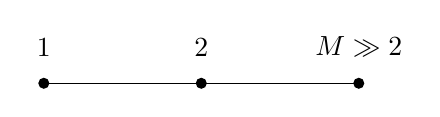
\begin{tikzpicture}
\draw (0,0)--(2,0)--(4,0);
\foreach \x/\lab in {0/1,2/2,4/{M\gg2}}{\fill (\x,0) circle (2pt);\node[above=6pt] at (\x,0){$\lab$};}
\end{tikzpicture}\par\small 图1
\end{center}
若将择劣删除贪心算法用于最大化问题，或将择优加入贪心算法用于最小化问题，则比值
\[\frac{G(E,\F,c)}{\operatorname{OPT}(E,\F,c)}\]
不存在正的统一下界或有限的统一上界。只需对图1所示简单图，考虑求最大权极小顶点覆盖，或最小权极大独立集。

但对于拟阵，使用哪一种贪心算法并无区别：由于所有基的基数相同，$(E,\F,c)$ 的最小化问题等价于 $(E,\F,c')$ 的最大化问题，其中 $c'(e):=M-c(e)$，$M:=1+\max\{c(e):e\in E\}$。因此 Kruskal 算法能最优地求解最小生成树问题。

Edmonds--Rado 定理20还给出了最大化问题中最优 $k$ 元解的如下刻画。
\st{定理22} 设 $(E,\F)$ 是拟阵，$c:E\to\R$，$k\in\N$，$X\in\F$ 且 $|X|=k$。则 $c(X)=\max\{c(Y):Y\in\F,|Y|=k\}$ 当且仅当以下两个条件成立：
\begin{enumerate}[label=(\alph*)]
\item 对所有满足 $X\cup\{y\}\notin\F$ 的 $y\in E\setminus X$ 以及所有 $x\in C(X,y)$，有 $c(x)\ge c(y)$；
\end{enumerate}

\begin{enumerate}[label=(\alph*),start=2]
\item 对所有满足 $X\cup\{y\}\in\F$ 的 $y\in E\setminus X$ 以及所有 $x\in X$，有 $c(x)\ge c(y)$。
\end{enumerate}
\pr 必要性显然：若某个 $y,x$ 违反其中一个条件，则 $k$ 元集 $X':=(X\cup\{y\})\setminus\{x\}\in\F$ 的费用大于 $X$。
证明充分性。令 $\F':=\{F\in\F:|F|\le k\}$。注意，截断之后的 $(E,\F')$ 仍然是拟阵。由于我们比较的是固定 $k$ 元集合上的最大化问题，所以可以对权重进行统一平移。具体地，令所有 $e\in E$ 的 $c'(e):=c(e)+M$，其中 $M=\max\{|c(e)|:e\in E\}$。将 $E=\{e_1,\ldots,e_n\}$ 排序，使 $c'(e_1)\ge\cdots\ge c'(e_n)$，且对任意 $i$，若 $c'(e_i)=c'(e_{i+1})$、$e_{i+1}\in X$，则 $e_i\in X$（即相同权重中 $X$ 的元素优先）。

设 $X'$ 是按此顺序对实例 $(E,\F',c')$ 运行择优加入贪心算法所得的解。由于 $(E,\F')$ 是拟阵，由定理20，
\begin{align*}
c(X')+kM&=c'(X')=\max\{c'(Y):Y\in\F'\}\\
&=\max\{c(Y):Y\in\F,|Y|=k\}+kM.
\end{align*}
最后证明 $X=X'$。已知 $|X|=k=|X'|$。若不同，取 $e_i\in X'\setminus X$，使 $i$ 最小。则 $X\cap\{e_1,\ldots,e_{i-1}\}=X'\cap\{e_1,\ldots,e_{i-1}\}$。若 $X\cup\{e_i\}\notin\F$，由(a)得 $C(X,e_i)\subseteq X'$，矛盾。若 $X\cup\{e_i\}\in\F$，由(b)得 $X\subseteq X'$，也不可能。\qed
将上述结论用于图拟阵，可得最小生成树的如下最优性条件。
\st{推论23（原书定理6.2的一部分）} 设 $G$ 是连通无向图，$c:E(G)\to\R$，$T$ 是 $G$ 的一棵生成树。则下列命题等价：
\begin{enumerate}[label=(\alph*)]
\item $T$ 是最小权生成树。
\item 对每条边 $e=\{u,v\}\in E(G)\setminus E(T)$，$T$ 中唯一的 $u$--$v$ 路上的每条边 $f$ 都满足 $c(f)\le c(e)$。
\end{enumerate}
\pr 对图拟阵 $M(G)$、权函数 $-c$ 及 $k=r(E(G))=|V(G)|-1$ 应用定理22。此时 $k$ 元独立集恰为生成树的边集。由于 $E(T)$ 已是基，条件(b)自动成立；而对每条非树边 $e=\{u,v\}$，$C(E(T),e)$ 由 $e$ 及 $T$ 中的 $u$--$v$ 路组成，故条件(a)恰为 $-c(f)\ge-c(e)$，即上述条件(b)。\qed

下面考虑同时满足两个或多个独立性条件的情形。
\sect{5\quad 拟阵交}
\st{定义24} 给定两个独立系统 $(E,\F_1)$ 和 $(E,\F_2)$，定义它们的\textbf{交}为 $(E,\F_1\cap\F_2)$。
有限个独立系统之交可类似定义。显然所得仍是独立系统。
\st{命题25} 任意独立系统 $(E,\F)$ 都是有限个拟阵之交。
\pr 由定理11，$(E,\F)$ 的每个回路 $C$ 都定义一个拟阵 $(E,\{F\subseteq E:C\setminus F\ne\varnothing\})$。该拟阵的独立集族不含 $C$，但是包含 $\F$ 中的所有元素。这些拟阵之交当然就是 $(E,\F)$。\qed
因为拟阵之交一般不是拟阵，不能期望用贪心算法求得最优公共独立集。但下述结论结合定理19，可以界定择优加入贪心算法所得解的质量。
\st{命题26} 若 $(E,\F)$ 是 $p$ 个拟阵之交，则 $q(E,\F)\ge1/p$。
\par\noindent\textbf{证明1。}由定理11(b)，对任意 $X\in\F$ 和 $e\in E$，$X\cup\{e\}$ 至多包含 $p$ 个回路。现由定理8即得结论。\qed

\par\noindent\textbf{证明2。}设 $\F=\bigcap_{i=1}^p\F_i$，其中 $(E,\F_i)$ 都是拟阵。任取 $S\subseteq E$ 及其在 $(E,\F)$ 中的两个基 $J,K$，只需证明 $|K|\le p|J|$。对每个 $i$，将 $J$ 扩充为 $J\cup K$ 在 $(E,\F_i)$ 中的一个基 $B_i$。由于 $K\in\F_i$，有 $|B_i|\ge|K|$。

任意 $e\in K\setminus J$ 不可能属于所有 $B_i$；否则 $J\cup\{e\}\subseteq B_i$ 对所有 $i$ 成立，从而 $J\cup\{e\}\in\F$，与 $J$ 的极大性矛盾。因此，每个 $e\in K\setminus J$ 至多属于 $p-1$ 个集合 $B_i\setminus J$，故
\[\sum_{i=1}^p|B_i\setminus J|\le(p-1)|K\setminus J|\le(p-1)|K|.\]
由 $J\subseteq B_i$，得到
\[p|K|\le\sum_{i=1}^p|B_i|=p|J|+\sum_{i=1}^p|B_i\setminus J|\le p|J|+(p-1)|K|.\]
移项即得 $|K|\le p|J|$，所以 $q(E,\F)\ge1/p$。\qed
由两个拟阵之交构成的独立系统尤其值得关注。一个例子是二分图 $G=(A\mathbin{\dot\cup}B,E(G))$ 中的匹配问题。若 $E=E(G)$，$\F:=\{F\subseteq E:F\text{ 是 }G\text{ 中的匹配}\}$，则 $(E,\F)$ 是两个拟阵之交。具体地，令
\[\F_1:=\{F\subseteq E:|\delta_F(x)|\le1\text{ 对所有 }x\in A\},\]
\[\F_2:=\{F\subseteq E:|\delta_F(x)|\le1\text{ 对所有 }x\in B\}.\]
由命题4(c)，$(E,\F_1)$、$(E,\F_2)$ 都是拟阵。显然 $\F=\F_1\cap\F_2$。


现在描述 Edmonds 用来求解以下问题的算法。
\alg{拟阵交问题}
\textbf{实例：}由独立性预言机给出的两个拟阵 $(E,\F_1)$、$(E,\F_2)$。\par
\textbf{任务：}求 $F\in\F_1\cap\F_2$，使 $|F|$ 最大。

从下述引理开始。回忆：对 $X\in\F$、$e\in E$，若 $X\cup\{e\}\notin\F$，$C(X,e)$ 表示其中唯一的回路；否则 $C(X,e)=\varnothing$。
\st{引理27（Frank [1981]）} 设 $(E,\F)$ 是拟阵，$X\in\F$。设 $x_1,\ldots,x_s\in X$，$y_1,\ldots,y_s\notin X$，满足：
\begin{enumerate}[label=(\alph*)]
\item 对 $k=1,\ldots,s$，$x_k\in C(X,y_k)$；
\item 对 $1\le j<k\le s$，$x_j\notin C(X,y_k)$。
\end{enumerate}
则 $(X\setminus\{x_1,\ldots,x_s\})\cup\{y_1,\ldots,y_s\}\in\F$。
\pr 令 $X_r:=(X\setminus\{x_1,\ldots,x_r\})\cup\{y_1,\ldots,y_r\}$，归纳证明所有 $X_r\in\F$。$r=0$ 显然。假设 $X_{r-1}\in\F$。若 $X_{r-1}\cup\{y_r\}\in\F$，立即得 $X_r\in\F$；否则由定理11(b)，$X_{r-1}\cup\{y_r\}$ 包含唯一回路 $C$。由(b)，$C(X,y_r)\subseteq X_{r-1}\cup\{y_r\}$，所以 $C=C(X,y_r)$。再由(a)，$x_r\in C$，故 $X_r=(X_{r-1}\cup\{y_r\})\setminus\{x_r\}\in\F$。\qed
Edmonds 拟阵交算法的思想如下：从 $X=\varnothing$ 出发，每次迭代使 $X$ 增加一个元素。一般不能指望存在 $e$ 使 $X\cup\{e\}\in\F_1\cap\F_2$，因此寻找“交错路”。为此定义辅助图。将 $C(X,e)$ 用于 $(E,\F_i)$ 时记作 $C_i(X,e)$（$i=1,2$）。

\begin{center}
\begin{tikzpicture}[>=Stealth,scale=.82]
\draw (0,0) ellipse (.48 and 2.15);\draw (3.5,0) ellipse (.48 and 2.15);
\node at (0,2.5){$X$};\node at (3.5,2.5){$E\setminus X$};
\foreach \y in {.55,1.6}{\draw[->](3.5,\y)--(0,\y);}
\foreach \y in {-.55,-1.6}{\draw[->](0,\y)--(3.5,\y);}
\draw (3.1,1.05)--(3.9,1.05);\draw(3.1,-1.05)--(3.9,-1.05);
\node at (4.25,1.6){$S_X$};\node at (4.25,-1.6){$T_X$};
\node at (1.75,1.05){$A_X^{(2)}$};\node at (1.75,-1.05){$A_X^{(1)}$};
\end{tikzpicture}\par\small 图2
\end{center}
给定 $X\in\F_1\cap\F_2$，定义有向辅助图 $G_X$：
\begin{align*}
A_X^{(1)}&:=\{(x,y):y\in E\setminus X,\ x\in C_1(X,y)\setminus\{y\}\},\\
A_X^{(2)}&:=\{(y,x):y\in E\setminus X,\ x\in C_2(X,y)\setminus\{y\}\},\\
G_X&:=(E,A_X^{(1)}\cup A_X^{(2)}).
\end{align*}
令
\[S_X:=\{y\in E\setminus X:X\cup\{y\}\in\F_1\},\qquad
T_X:=\{y\in E\setminus X:X\cup\{y\}\in\F_2\},\]
见图2，并寻找从 $S_X$ 到 $T_X$ 的最短路。这样的路使我们能够扩充 $X$。（若 $S_X\cap T_X\ne\varnothing$，就有长度为0的路，可将交集中的任一元素加入 $X$。）
\st{引理28} 设 $X\in\F_1\cap\F_2$。设 $y_0,x_1,y_1,\ldots,x_s,y_s$ 依次为 $G_X$ 中一条最短 $y_0$--$y_s$ 路的顶点，且 $y_0\in S_X$、$y_s\in T_X$。则
\[X':=(X\cup\{y_0,\ldots,y_s\})\setminus\{x_1,\ldots,x_s\}\in\F_1\cap\F_2.\]
\pr 首先说明 $X\cup\{y_0\}$、$x_1,\ldots,x_s$ 和 $y_1,\ldots,y_s$ 对 $\F_1$ 满足引理27。因为 $y_0\in S_X$，有 $X\cup\{y_0\}\in\F_1$。因所有 $(x_j,y_j)\in A_X^{(1)}$，(a)成立；(b)也成立，否则可对路取捷径。因此 $X'\in\F_1$。
其次，$X\cup\{y_s\}$、$x_s,x_{s-1},\ldots,x_1$ 和 $y_{s-1},\ldots,y_1,y_0$ 对 $\F_2$ 满足引理27。因为 $y_s\in T_X$，有 $X\cup\{y_s\}\in\F_2$。因所有 $(y_{j-1},x_j)\in A_X^{(2)}$，(a)成立；而(b)成立，因为否则可对路取捷径。

所以 $X'\in\F_2$。\qed
下面证明：若 $G_X$ 中没有 $S_X$--$T_X$ 路，则 $X$ 已经具有最大基数。需要以下简单事实。
\st{命题29} 设 $(E,\F_1)$、$(E,\F_2)$ 是两个拟阵，秩函数分别为 $r_1,r_2$。则对任意 $F\in\F_1\cap\F_2$、$Q\subseteq E$，
\[|F|\le r_1(Q)+r_2(E\setminus Q).\]
\pr $F\cap Q\in\F_1$ 蕴含 $|F\cap Q|\le r_1(Q)$；同样 $F\setminus Q\in\F_2$ 蕴含 $|F\setminus Q|\le r_2(E\setminus Q)$。两式相加即得。\qed
\st{引理30} $X\in\F_1\cap\F_2$ 的基数最大，当且仅当 $G_X$ 中不存在 $S_X$--$T_X$ 路。
\pr 若存在这样的路，则也存在最短的一条。应用引理28，即得基数更大的 $X'\in\F_1\cap\F_2$。
\begin{center}
\begin{tikzpicture}[>=Stealth,scale=.82]
\draw (0,0) ellipse (.48 and 2.15);\draw (3.5,0) ellipse (.48 and 2.15);
\node at(0,2.5){$X$};\node at(3.5,2.5){$E\setminus X$};
\foreach \y in {.55,1.6}{\draw[->](3.5,\y)--(0,\y);}
\foreach \y in {-.55,-1.6}{\draw[->](0,\y)--(3.5,\y);}
\draw[->](3.5,-.15)--(0,1.05);\draw[->](0,-1.05)--(3.5,.85);
\draw(3.1,1.05)--(3.9,1.05);\draw(3.1,-1.05)--(3.9,-1.05);
\draw[dashed](-1.1,-.32)--(4.6,.32);
\node at(-.85,0){$R$};\node at(-.9,-.62){$E\setminus R$};
\node at(4.25,1.6){$S_X$};\node at(4.25,-1.6){$T_X$};
\node at(1.75,1.05){$A_X^{(2)}$};\node at(1.75,-1.05){$A_X^{(1)}$};
\end{tikzpicture}\par\small 图3
\end{center}
否则，设 $R$ 是 $G_X$ 中从 $S_X$ 可达的顶点集（见图3），则 $R\cap T_X=\varnothing$。以 $r_1,r_2$ 分别表示 $\F_1,\F_2$ 的秩函数。
断言 $r_2(R)=|X\cap R|$。否则存在 $y\in R\setminus X$，使 $(X\cap R)\cup\{y\}\in\F_2$。由于 $y\notin T_X$，$X\cup\{y\}\notin\F_2$，所以回路 $C_2(X,y)$ 必包含某个 $x\in X\setminus R$。但 $(y,x)\in A_X^{(2)}$ 意味着有边离开 $R$，与 $R$ 的定义矛盾。

再证 $r_1(E\setminus R)=|X\setminus R|$。否则存在 $y\in(E\setminus R)\setminus X$，使 $(X\setminus R)\cup\{y\}\in\F_1$。由于 $y\notin S_X$，$X\cup\{y\}\notin\F_1$，所以回路 $C_1(X,y)$ 必包含某个 $x\in X\cap R$。但 $(x,y)\in A_X^{(1)}$ 意味着有边离开 $R$，与 $R$ 的定义矛盾。
综上，$|X|=r_2(R)+r_1(E\setminus R)$。由命题29，$X$ 最优。\qed
这一证明的最后部分给出如下极小极大等式。
\st{定理31（Edmonds [1970]）} 设 $(E,\F_1)$、$(E,\F_2)$ 是两个拟阵，其秩函数为 $r_1,r_2$。则
\[\max\{|X|:X\in\F_1\cap\F_2\}=\min\{r_1(Q)+r_2(E\setminus Q):Q\subseteq E\}.\quad\square\]
现在可以详细描述算法。
\alg{Edmonds 拟阵交算法}
\textbf{输入：}由独立性预言机给出的两个拟阵 $(E,\F_1)$、$(E,\F_2)$。\par
\textbf{输出：}基数最大的集合 $X\in\F_1\cap\F_2$。
\begin{enumerate}[label=\arabic*.]
\item 令 $X:=\varnothing$。
\item 对每个 $y\in E\setminus X$ 和 $i\in\{1,2\}$，计算
\[C_i(X,y):=\{x\in X\cup\{y\}:X\cup\{y\}\notin\F_i,\ (X\cup\{y\})\setminus\{x\}\in\F_i\}.\]
\item 按前面的定义计算 $S_X,T_X,G_X$。
\item 用广度优先搜索（BFS）在 $G_X$ 中寻找最短 $S_X$--$T_X$ 路 $P$。若不存在则停止。
\item 令 $X:=X\mathbin{\triangle}V(P)$，返回步骤2。
\end{enumerate}
\st{定理32} Edmonds 拟阵交算法在 $O(|E|^3\theta)$ 时间内正确求解拟阵交问题，其中 $\theta$ 是两种独立性预言机复杂度的最大值。
\pr 正确性来自引理28、30。步骤2、3可在 $O(|E|^2\theta)$ 时间内完成，步骤4可在 $O(|E|)$ 时间内完成。由于增广次数至多 $|E|$，总复杂度为 $O(|E|^3\theta)$。\qed

上述算法可以推广到带权情形，仍然能得到最优解。

\sect{6\quad 拟阵划分}
现在不再考虑拟阵的交，而考虑按如下方式定义的并。
\st{定义33} 设 $(E,\F_1),\ldots,(E,\F_k)$ 是 $k$ 个拟阵。若存在划分 $X=X_1\mathbin{\dot\cup}\cdots\mathbin{\dot\cup}X_k$，使 $X_i\in\F_i$（$i=1,\ldots,k$），则称 $X\subseteq E$ \textbf{可划分}。令 $\F$ 为 $E$ 的可划分子集族，则称 $(E,\F)$ 为这些拟阵的\textbf{并}或\textbf{和}。
我们将证明拟阵的并仍是拟阵，并通过拟阵交求解下列问题。
\alg{拟阵划分问题}
\textbf{实例：}数 $k\in\N$，以及由独立性预言机给出的 $k$ 个拟阵 $(E,\F_1),\ldots,(E,\F_k)$。\par
\textbf{任务：}求基数最大的可划分集合 $X\subseteq E$。
关于拟阵划分的主要定理是：
\st{定理34（Nash-Williams [1967]）} 设 $(E,\F_1),\ldots,(E,\F_k)$ 是拟阵，其秩函数为 $r_1,\ldots,r_k$；设 $(E,\F)$ 是它们的并。则 $(E,\F)$ 是拟阵，其秩函数为
\[r(X)=\min_{A\subseteq X}\left(|X\setminus A|+\sum_{i=1}^kr_i(A)\right).\]
\pr $(E,\F)$ 显然是独立系统。我们先验证这一独立系统的秩满足上述公式，再证明该秩函数次模，从而由定理10的秩判别法得到 $(E,\F)$ 是拟阵。为此，先设 $X\subseteq E$。任取可划分的 $Y\subseteq X$，即 $Y=Y_1\mathbin{\dot\cup}\cdots\mathbin{\dot\cup}Y_k$ 且 $Y_i\in\F_i$，以及任意 $A\subseteq X$，都有
\[|Y|=|Y\setminus A|+|Y\cap A|\le|X\setminus A|+\sum_{i=1}^k|Y_i\cap A|
\le|X\setminus A|+\sum_{i=1}^kr_i(A).\]
所以 $r(X)\le\min_{A\subseteq X}(|X\setminus A|+\sum_i r_i(A))$。

另一方面，令 $X':=X\times\{1,\ldots,k\}$，在其上定义两个拟阵。对 $Q\subseteq X'$ 和 $i\in\{1,\ldots,k\}$，记 $Q_i:=\{e\in X:(e,i)\in Q\}$。令
\[\mathcal I_1:=\{Q\subseteq X':Q_i\in\F_i\text{ 对所有 }i=1,\ldots,k\},\]
\[\mathcal I_2:=\{Q\subseteq X':Q_i\cap Q_j=\varnothing\text{ 对所有 }i\ne j\}.\]
显然 $(X',\mathcal I_1)$ 和 $(X',\mathcal I_2)$ 都是拟阵，其秩函数分别为
\[s_1(Q):=\sum_{i=1}^kr_i(Q_i),\qquad s_2(Q):=\left|\bigcup_{i=1}^kQ_i\right|\quad(Q\subseteq X').\]

现在 $X$ 的可划分子集族可写成
\[\{A\subseteq X:\text{存在 }f:A\to\{1,\ldots,k\},\ \{(e,f(e)):e\in A\}\in\mathcal I_1\cap\mathcal I_2\}.\]
所以可划分集合的最大基数，等于 $\mathcal I_1$ 和 $\mathcal I_2$ 中公共独立集的最大基数。由定理31，该值为 $\min\{s_1(Q)+s_2(X'\setminus Q):Q\subseteq X'\}$。若 $Q$ 达到此最小值，令 $A:=Q_1\cap\cdots\cap Q_k$，则
\begin{align*}
r(X)&=s_1(Q)+s_2(X'\setminus Q)\\
&=\sum_{i=1}^kr_i(Q_i)+\left|X\setminus\bigcap_{i=1}^kQ_i\right|
\ge\sum_{i=1}^kr_i(A)+|X\setminus A|.
\end{align*}
于是找到了满足 $\sum_i r_i(A)+|X\setminus A|\le r(X)$ 的 $A\subseteq X$。

证明秩公式后，最后证明 $r$ 次模；由定理10即知 $(E,\F)$ 是拟阵。设 $X,Y\subseteq E$，取 $A\subseteq X$、$B\subseteq Y$，满足 $r(X)=|X\setminus A|+\sum_i r_i(A)$、$r(Y)=|Y\setminus B|+\sum_i r_i(B)$。则
\begin{align*}
r(X)+r(Y)&=|X\setminus A|+|Y\setminus B|+\sum_{i=1}^k(r_i(A)+r_i(B))\\
&\ge|(X\cup Y)\setminus(A\cup B)|+|(X\cap Y)\setminus(A\cap B)|\\
&\quad+\sum_{i=1}^k(r_i(A\cup B)+r_i(A\cap B))\\
&\ge r(X\cup Y)+r(X\cap Y).
\end{align*}\qed
上述证明中的构造（Edmonds [1970]）将拟阵划分问题归约为拟阵交问题。反向归约也能做到（原书第13章习题20），所以可把二者看作等价问题。

注意，我们能在任意多个拟阵的并中寻找最大独立集，而超过两个拟阵的交则难以处理。
